% Scenario tree
% Author: Rasmus Pank Roulund
\documentclass{minimal}
\usepackage{tikz}
\usepackage{verbatim}


\usetikzlibrary{shapes}
\usepackage{amsmath}
\usepackage{xspace}
\newcommand{\A}{\ensuremath{\mathcal{A}}\xspace}
\newcommand{\B}{\ensuremath{\mathcal{B}}\xspace}
\newcommand\pa[1]{\ensuremath{\left(#1\right)}}
\begin{document}
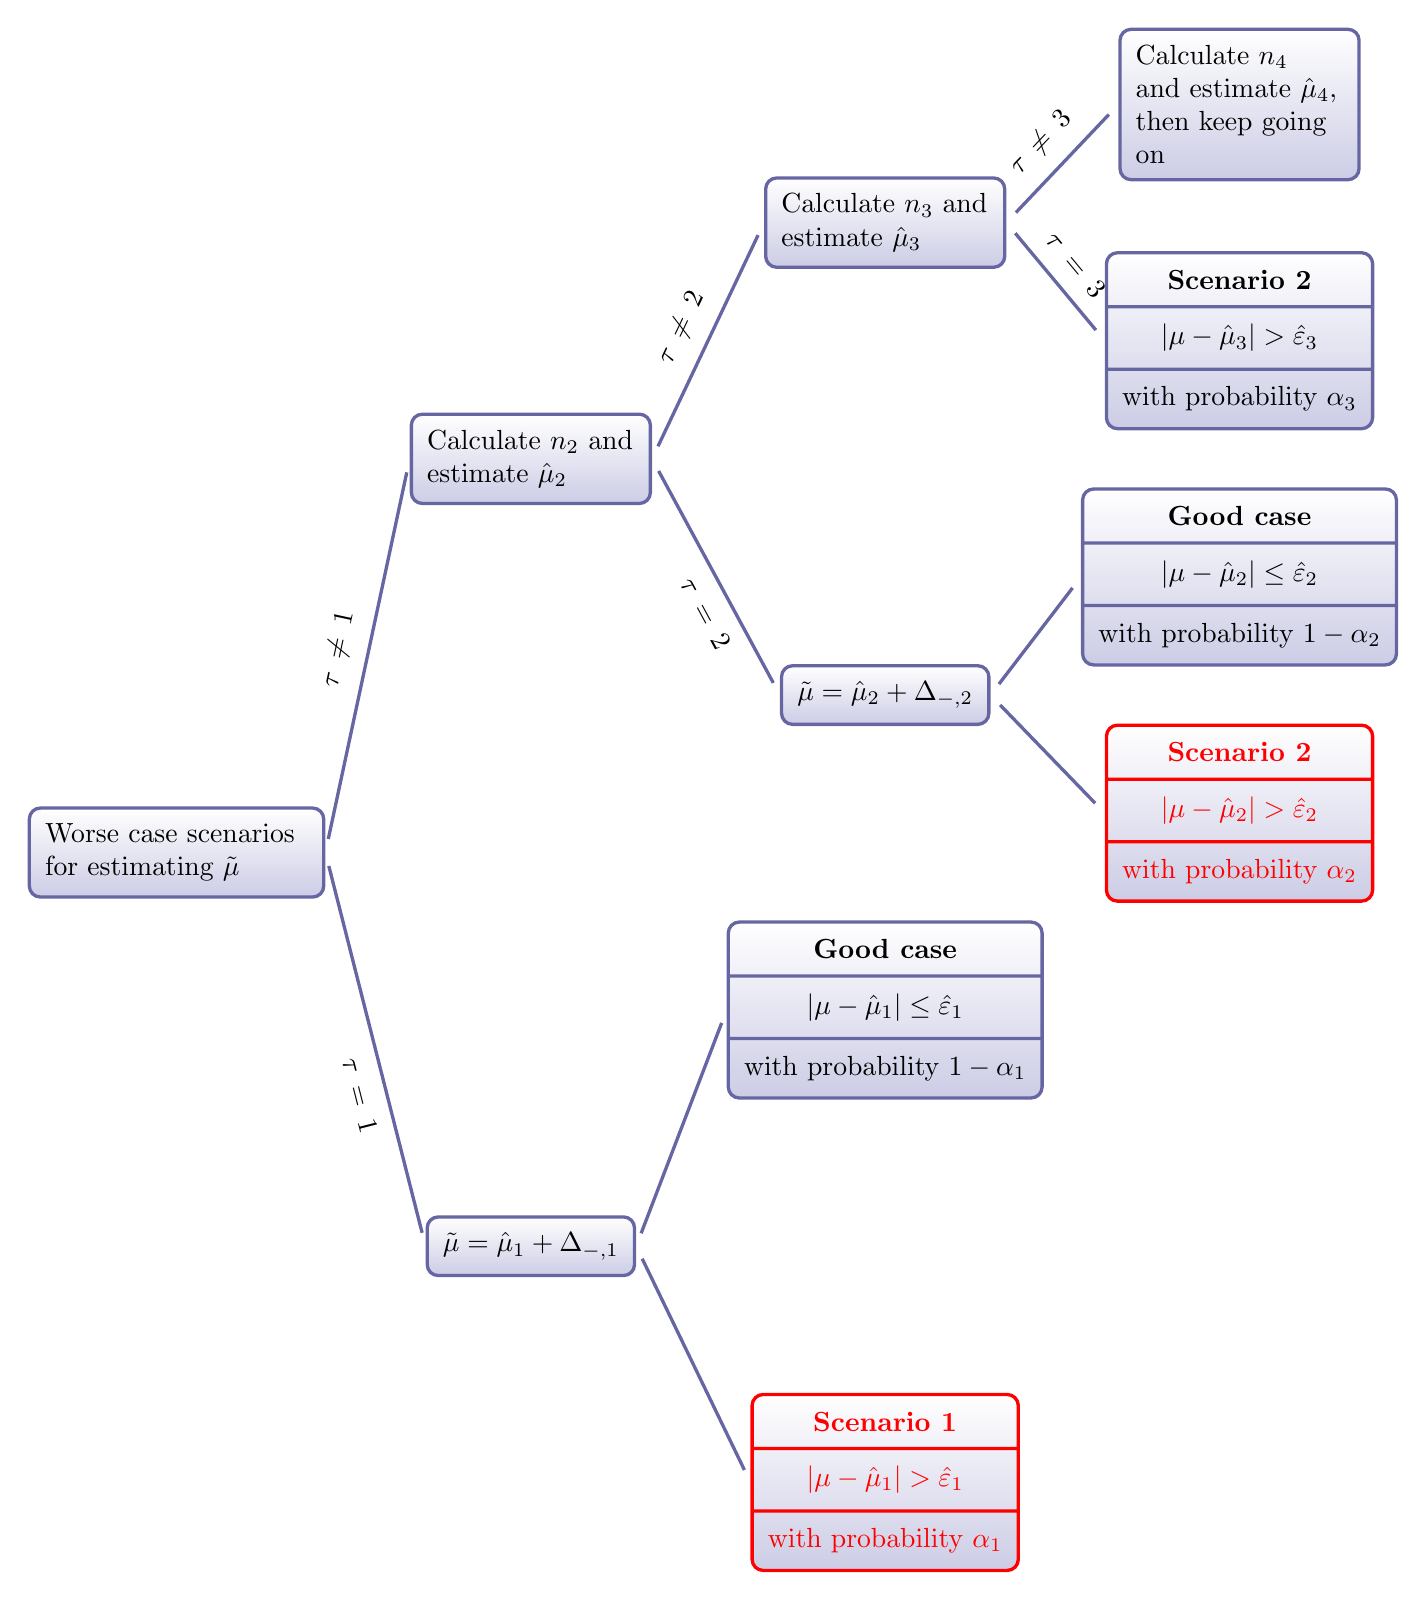
\begin{tikzpicture}[
    grow=right,
    level 1/.style={sibling distance=10cm,level distance=4.5cm},
    level 2/.style={sibling distance=6cm, level distance=4.5cm},
        level 3/.style={sibling distance=3cm, level distance=4.5cm},
    edge from parent/.style={very thick,draw=blue!40!black!60,
        shorten >=5pt, shorten <=5pt},
    edge from parent path={(\tikzparentnode.east) -- (\tikzchildnode.west)},
    kant/.style={text width=2cm, text centered, sloped},
    every node/.style={text ragged, inner sep=2mm},
    punkt/.style={rectangle, rounded corners, shade, top color=white,
    bottom color=blue!50!black!20, draw=blue!40!black!60, very
    thick }
    ]

\node[punkt, text width=9.5em] {Worse case scenarios for estimating $\tilde{\mu}$}
    %Lower part lv1
    child {
        node[punkt] { $\tilde{\mu}=\hat{\mu}_1+\Delta_{-,1}$ }
child{node[punkt] [rectangle split,color=red, rectangle split, rectangle split parts=3,
         text ragged]{ \textbf{Scenario  1}
                  \nodepart{second}
            $|{\mu-\hat{\mu}_1}| >\hat{\varepsilon}_1$
                          \nodepart{third}
            with probability $\alpha_1$}       
%             edge from parent
%            node[kant, below, pos=.6] {bad case}
            }
            child{node[punkt] [rectangle split, rectangle split, rectangle split parts=3,
         text ragged]{ \textbf{Good case}
                  \nodepart{second}
            $|{\mu-\hat{\mu}_1}| \leq\hat{\varepsilon}_1$
                          \nodepart{third}
            with probability $1-\alpha_1$}       
%             edge from parent
%            node[kant, below, pos=.6] {good case}
            }
        edge from parent
            node[kant, below, pos=.6] {$\tau =1$}
    }
    %Upper part, lv1
    child {
        node[punkt, text width=7.5em] {Calculate $n_2$ and estimate $\hat{\mu}_2$}
        %child 1
        child {
            node [punkt] { $\tilde{\mu}=\hat{\mu}_2+\Delta_{-,2}$ }
            child{node[punkt,color=red,rectangle split, rectangle split,
            rectangle split parts=3]{ \textbf{Scenario 2}
                \nodepart{second}
     $|{\mu-\hat{\mu}_2}| >\hat{\varepsilon}_2$
                  \nodepart{third}
            with probability $\alpha_2$}}
           child{node[punkt,rectangle split, rectangle split,
            rectangle split parts=3]{ \textbf{Good case}
                \nodepart{second}
     $|{\mu-\hat{\mu}_2}| \leq\hat{\varepsilon}_2$
                  \nodepart{third}
            with probability $1-\alpha_2$}}
            edge from parent
                node[below, kant,  pos=.6] {$\tau = 2$}
        }
        %child 2
	        child {    node[punkt, text width=7.5em] {Calculate $n_3$ and estimate $\hat{\mu}_3$}
	        child{
	            node [punkt, rectangle split, rectangle split parts=3]{
	                \textbf{Scenario 2}
	                \nodepart{second}
	     $|{\mu-\hat{\mu}_3}| >\hat{\varepsilon}_3$
	                  \nodepart{third}
            with probability $\alpha_3$
            }
            edge from parent
                node[kant, above] {$\tau=3$}}                
                 child{
	            node [punkt, text width=7.5em]{Calculate $n_4$ and estimate $\hat{\mu}_4$, then keep going on}
            edge from parent
                node[kant, above] {$\tau\neq3$}}
                   edge from parent{
                node[kant, above] {$\tau \neq 2$}}      
                }                
            edge from parent{
                node[kant, above] {$\tau \neq 1$}}
    };
\end{tikzpicture}
\end{document}